\chapter{光照(Lighting)}
\begin{flushleft}
考虑图\ref{fig:8-1}。 在左边我们有一个没有照明的球体,在右边,我们有一个点亮的球体。 正如你所看到的,左边的球体看起来很平坦——也许它根本不是一个球体,而只是一个2D圆圈! 另一方面,右侧的球体确实看起来是3D——照明和阴影有助于我们对物体的固体形状和体积的感知。 事实上,我们对世界的视觉感知取决于光线及其与材料的相互作用,因此,产生逼真场景的大部分问题都与物理上精确的照明模型有关。
\end{flushleft}

\begin{figure}[h]
    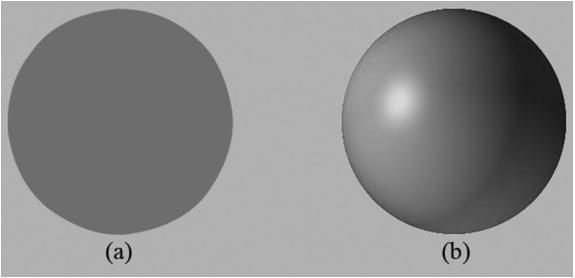
\includegraphics[width=\textwidth]{8-1}
    \centering
    \caption{(a)未点亮的球体看起来是2D。(b)点亮的球体看起来是3D。}
    \label{fig:8-1}
\end{figure}

\begin{flushleft}
当然,一般来说,模型越准确,计算成本越高; 因此,必须在现实主义和速度之间达成平衡。 例如,用于电影的3D特殊FX场景可以比游戏更复杂并且使用非常逼真的照明模型,因为电影的帧是预渲染的,因此它们可以花费数小时或数天来处理帧。 另一方面,游戏是实时应用程序,因此,帧需要以每秒至少30帧的速率绘制。\\
请注意,本书中解释和实现的照明模型很大程度上基于[Möller08]中描述的模型。\\
~\\
{\large Objectives:}
\begin{itemize}
    \item 了解灯光和材料之间的相互作用
    \item 了解局部照明和全局照明之间的差异
    \item 了解我们如何在数学上描述表面上的一个点“朝向”的方向,以便我们可以确定入射光照射到表面的角度
    \item 学习如何正确转换法向量
    \item 能够区分环境光,漫反射光和镜面光
    \item 了解如何实现定向灯,指示灯和聚光灯
    \item 通过控制衰减参数来了解如何根据深度改变光强度
\end{itemize}
\end{flushleft}

\section{光与材质的相互作用(Light And Meterial Interaction)}
\begin{flushleft}
使用灯光时,我们不再直接指定顶点颜色; 相反,我们指定材质和灯光,然后应用光照方程式,根据光/材料相互作用计算我们的顶点颜色。 这样可以使对象更加逼真地着色(再次比较图\ref{fig:8-1}a和\ref{fig:8-1}b)。\\
可以将材质视为确定光如何与对象表面相互作用的属性。 比如表面反射和吸收的光的颜色,表面下材料的折射率,表面的光滑程度以及表面的透明度。 通过指定材质属性,我们可以模拟不同类型的真实世界表面,如木材,石材,玻璃,金属和水。\\
在我们的模型中,光源可以发出各种强度的红色,绿色和蓝色光; 通过这种方式,我们可以模拟许多浅色。 当光从光源向外传播并与物体碰撞时,一些光可能被吸收而一些光可能被反射(对于透明物体,例如玻璃,一些光线穿过介质,但我们不考虑这里的透明度)。 反射光现在沿着其新的路径行进并且可能撞击其他物体,其中一些光再次被吸收和反射。 在完全吸收之前,光线可能会撞击许多物体。 据推测,一些光线最终会进入眼睛(见图\ref{fig:8-1})并撞击视网膜上的光受体细胞(称为视锥细胞和视杆细胞)。\\
\end{flushleft}

\begin{figure}[h]
    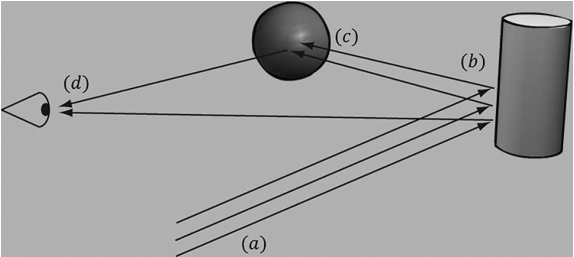
\includegraphics[width=\textwidth]{8-2}
    \centering
    \caption{(a)入射白光的通量。(b)光线照射到圆柱体上,一些光线被吸收,其他光线散射到眼睛和球体上。(c)从圆筒向球体反射的光被再次吸收或反射并进入眼睛。(d)眼睛接收入射光,确定眼睛看到的是什么。}
    \label{fig:8-2}
\end{figure}

